%%%%%%%%%%%%%%%%%%%%%%%%%%%%% Define Article %%%%%%%%%%%%%%%%%%%%%%%%%%%%%%%%%%
\documentclass{article}
%%%%%%%%%%%%%%%%%%%%%%%%%%%%%%%%%%%%%%%%%%%%%%%%%%%%%%%%%%%%%%%%%%%%%%%%%%%%%%%

%%%%%%%%%%%%%%%%%%%%%%%%%%%%% Using Packages %%%%%%%%%%%%%%%%%%%%%%%%%%%%%%%%%%
\usepackage{fancyhdr}
\usepackage{lastpage}
\usepackage{titling}
\usepackage[danish]{babel}
\usepackage{geometry}
\usepackage{graphicx}
\usepackage{amssymb}
\usepackage{amsmath}
\usepackage{amsthm}
\usepackage{empheq}
\usepackage{mdframed}
\usepackage{booktabs}
\usepackage{lipsum}
\usepackage{graphicx}
\usepackage{color}
\usepackage[dvipsnames]{xcolor}
\usepackage{psfrag}
\usepackage{pgfplots}
\usepackage{bm}
\usepackage{hyperref}
\usepackage{minted}
\usepackage{seqsplit}
\usepackage[backend=biber]{biblatex}
\addbibresource{refs.bib}
%%%%%%%%%%%%%%%%%%%%%%%%%%%%%%%%%%%%%%%%%%%%%%%%%%%%%%%%%%%%%%%%%%%%%%%%%%%%%%%

% Other Settings

%%%%%%%%%%%%%%%%%%%%%%%%%% Page Setting %%%%%%%%%%%%%%%%%%%%%%%%%%%%%%%%%%%%%%%
\geometry{a4paper, bottom=3cm}


%%%%%%%%%%%%%%%%%%%%%%%%%% Styles %%%%%%%%%%%%%%%%%%%%%%%%%%%%%%%%%%%%%%%%%%%%%
\usemintedstyle{borland}
%%%%%%%%%%%%%%%%%%%%%%%%%% Define some useful colors %%%%%%%%%%%%%%%%%%%%%%%%%%
\definecolor{ocre}{RGB}{243,102,25}
\definecolor{mygray}{RGB}{243,243,244}
\definecolor{deepGreen}{RGB}{26,111,0}
\definecolor{shallowGreen}{RGB}{235,255,255}
\definecolor{deepBlue}{RGB}{61,124,222}
\definecolor{shallowBlue}{RGB}{235,249,255}
%%%%%%%%%%%%%%%%%%%%%%%%%%%%%%%%%%%%%%%%%%%%%%%%%%%%%%%%%%%%%%%%%%%%%%%%%%%%%%%

%%%%%%%%%%%%%%%%%%%%%%%%%%% Define codecomment command %%%%%%%%%%%%%%%%%%%%%%%%
\newcommand{\code}[1]{\small\mintinline[xleftmargin=2em, xrightmargin=2em,
breaklines]{java}{#1}}
\newcommand{\class}[1]{\textcolor{BlueViolet}{\small\ttfamily\seqsplit{#1}}}
\newcommand{\method}[1]{\textcolor{Orange}{\small\ttfamily\seqsplit{#1}}}
\newcommand{\attribute}[1]{\textcolor{Purple}{\small\ttfamily\seqsplit{#1}}}
\newcommand{\snippet}[3]{\inputminted[firstline=#1,lastline=#2,linenos,
xleftmargin=1.5em, breaklines]{java}{#3}}
%%%%%%%%%%%%%%%%%%%%%%%%%%%%%%%%%%%%%%%%%%%%%%%%%%%%%%%%%%%%%%%%%%%%%%%%%%%%%%%

%%%%%%%%%%%%%%%%%%%%%%%%%% Define an orangebox command %%%%%%%%%%%%%%%%%%%%%%%%
\newcommand\orangebox[1]{\fcolorbox{ocre}{mygray}{\hspace{1em}#1\hspace{1em}}}
%%%%%%%%%%%%%%%%%%%%%%%%%%%%%%%%%%%%%%%%%%%%%%%%%%%%%%%%%%%%%%%%%%%%%%%%%%%%%%%

%%%%%%%%%%%%%%%%%%%%%%%%%%%% English Environments %%%%%%%%%%%%%%%%%%%%%%%%%%%%%
\newtheoremstyle{mytheoremstyle}{3pt}{3pt}{\normalfont}{0cm}{\rmfamily\bfseries}{}{1em}{{\color{black}\thmname{#1}~\thmnumber{#2}}\thmnote{\,--\,#3}}
\newtheoremstyle{myproblemstyle}{3pt}{3pt}{\normalfont}{0cm}{\rmfamily\bfseries}{}{1em}{{\color{black}\thmname{#1}~\thmnumber{#2}}\thmnote{\,--\,#3}}
\theoremstyle{mytheoremstyle}
\newmdtheoremenv[linewidth=1pt,backgroundcolor=shallowGreen,linecolor=deepGreen,leftmargin=0pt,innerleftmargin=20pt,innerrightmargin=20pt,]{theorem}{Theorem}[section]
\theoremstyle{mytheoremstyle}
\newmdtheoremenv[linewidth=1pt,backgroundcolor=shallowBlue,linecolor=deepBlue,leftmargin=0pt,innerleftmargin=20pt,innerrightmargin=20pt,]{definition}{Definition}[section]
\theoremstyle{myproblemstyle}
\newmdtheoremenv[linecolor=black,leftmargin=0pt,innerleftmargin=10pt,innerrightmargin=10pt,]{problem}{Problem}[section]
%%%%%%%%%%%%%%%%%%%%%%%%%%%%%%%%%%%%%%%%%%%%%%%%%%%%%%%%%%%%%%%%%%%%%%%%%%%%%%%

%%%%%%%%%%%%%%%%%%%%%%%%%%%%%%% Plotting Settings %%%%%%%%%%%%%%%%%%%%%%%%%%%%%
\usepgfplotslibrary{colorbrewer}
\pgfplotsset{width=8cm,compat=1.9}
%%%%%%%%%%%%%%%%%%%%%%%%%%%%%%%%%%%%%%%%%%%%%%%%%%%%%%%%%%%%%%%%%%%%%%%%%%%%%%%

%%%%%%%%%%%%%%%%%%%%%%%%%%%%%%% Title & Author %%%%%%%%%%%%%%%%%%%%%%%%%%%%%%%%
\title{\textbf{Objektorienteret Programmering Projekt PacMan}}
\author{Andreas K. L. \quad Aske W. F. \quad Magnus R. K.}
%%%%%%%%%%%%%%%%%%%%%%%%%%%%%%%%%%%%%%%%%%%%%%%%%%%%%%%%%%%%%%%%%%%%%%%%%%%%%%%

\begin{document}
\pagenumbering{gobble}
\begin{titlepage}
    \maketitle
    \begin{figure}[H]
        \begin{center}
            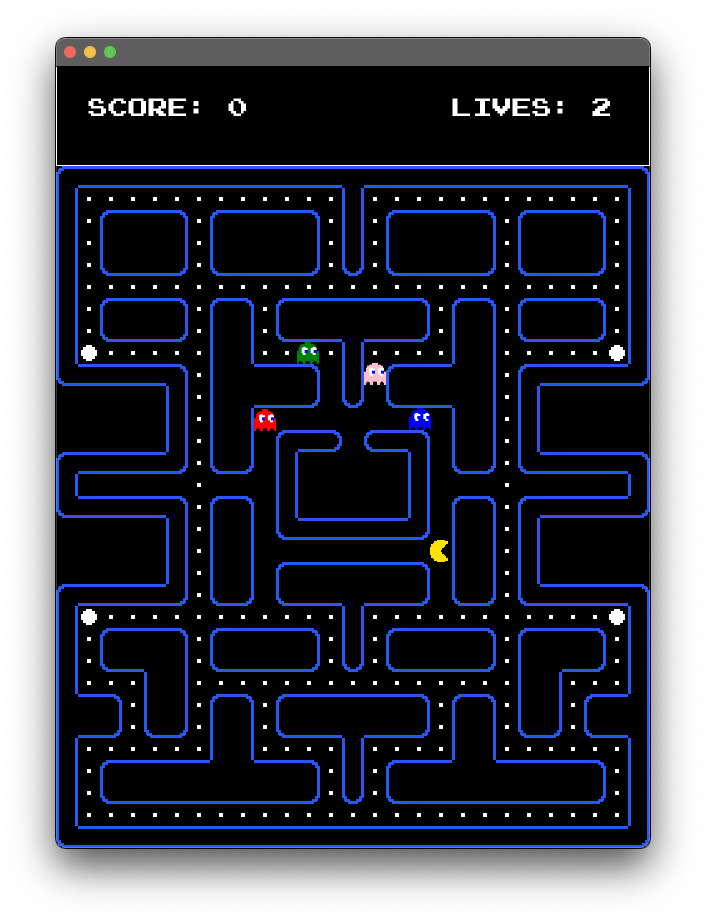
\includegraphics[width=0.77\textwidth]{figures/FrontPageImage.png}
        \end{center}
    \end{figure}
\end{titlepage}
    \clearpage
    \newpage
    \pagenumbering{arabic}
    \setcounter{page}{1}

    % Only footer, no header
    \pagestyle{fancy}
    % \fancyhf{} 
    \fancyfoot[C]{\textbf{\thepage}\ of \pageref{LastPage}}
    % \renewcommand{\headrulewidth}{0pt}  

    \tableofcontents
    \newpage
\section{Projektbeskrivelse}\label{sec:Beskrivelse} % (fold)

Til fordel for at sikre en så tro kopi til originalen som overhovedet muligt, er
dette projekts hovedformål, at udvikle spilfunktionalitet mht.
kravsspecifikationen. 

Der har været et tvetydigt krav, efter vores mening, som omhandler hvorledes
PacMan skal bevæge sig. Kravet lyder således at: PacMan skal bevæge sig
kontinuerligt i den regning han vender, og denne retning skal kunne styres via
tastetyk, f.eks. ved brug af piletasterne. Når PacMan støder mod en væg, skal
han forblive stationær indtil hans retning ændres.

Afvigelsen vi har gjort os med hensyn til dette krav er, at vi gerne ville
forbedre brugeroplevelsen i den forstand at man skal kunne bevæge omkring
hjørner uden at sidde fast. Beskrivelsen af implementeringen af denne ændring
kan ses i \autoref{sub:PacMan Kontrol}.

Udover dette nåede vi ikke kravet om at spøgelserne skal flygte fra PacMan når
han er i power stadiet.


% \begin{itemize}
%   \item Antag, at læseren af jeres rapport har læst kravsspecifikationen fra
%   projektbeskrivelsen i slutningen af dette dokument, og undlad at gentage
%   unødvendige detaljer derfra.
%   \item Formålet med denne sektion er at dokumentere eventuelle afvigelser fra
%   kravsspecifikationen.
%   \item Har I, for eksempel, gjort jer forsimplende antagelser ift.
%   specifikationen? Eller tolket eventuelle tvetydigheder i specifikationen?
%   Tilføjet nye krav? Beskriv hvilke og hvordan I evt. har tolket
%   specifikationen.
%   \item Hold det kort, især hvis I har få afvigelser.
% \end{itemize}
\newpage
% section Beskrivelse (end)

\section{Design}\label{sec:Design} % (fold)

\begin{figure}[H]
    \begin{center}
        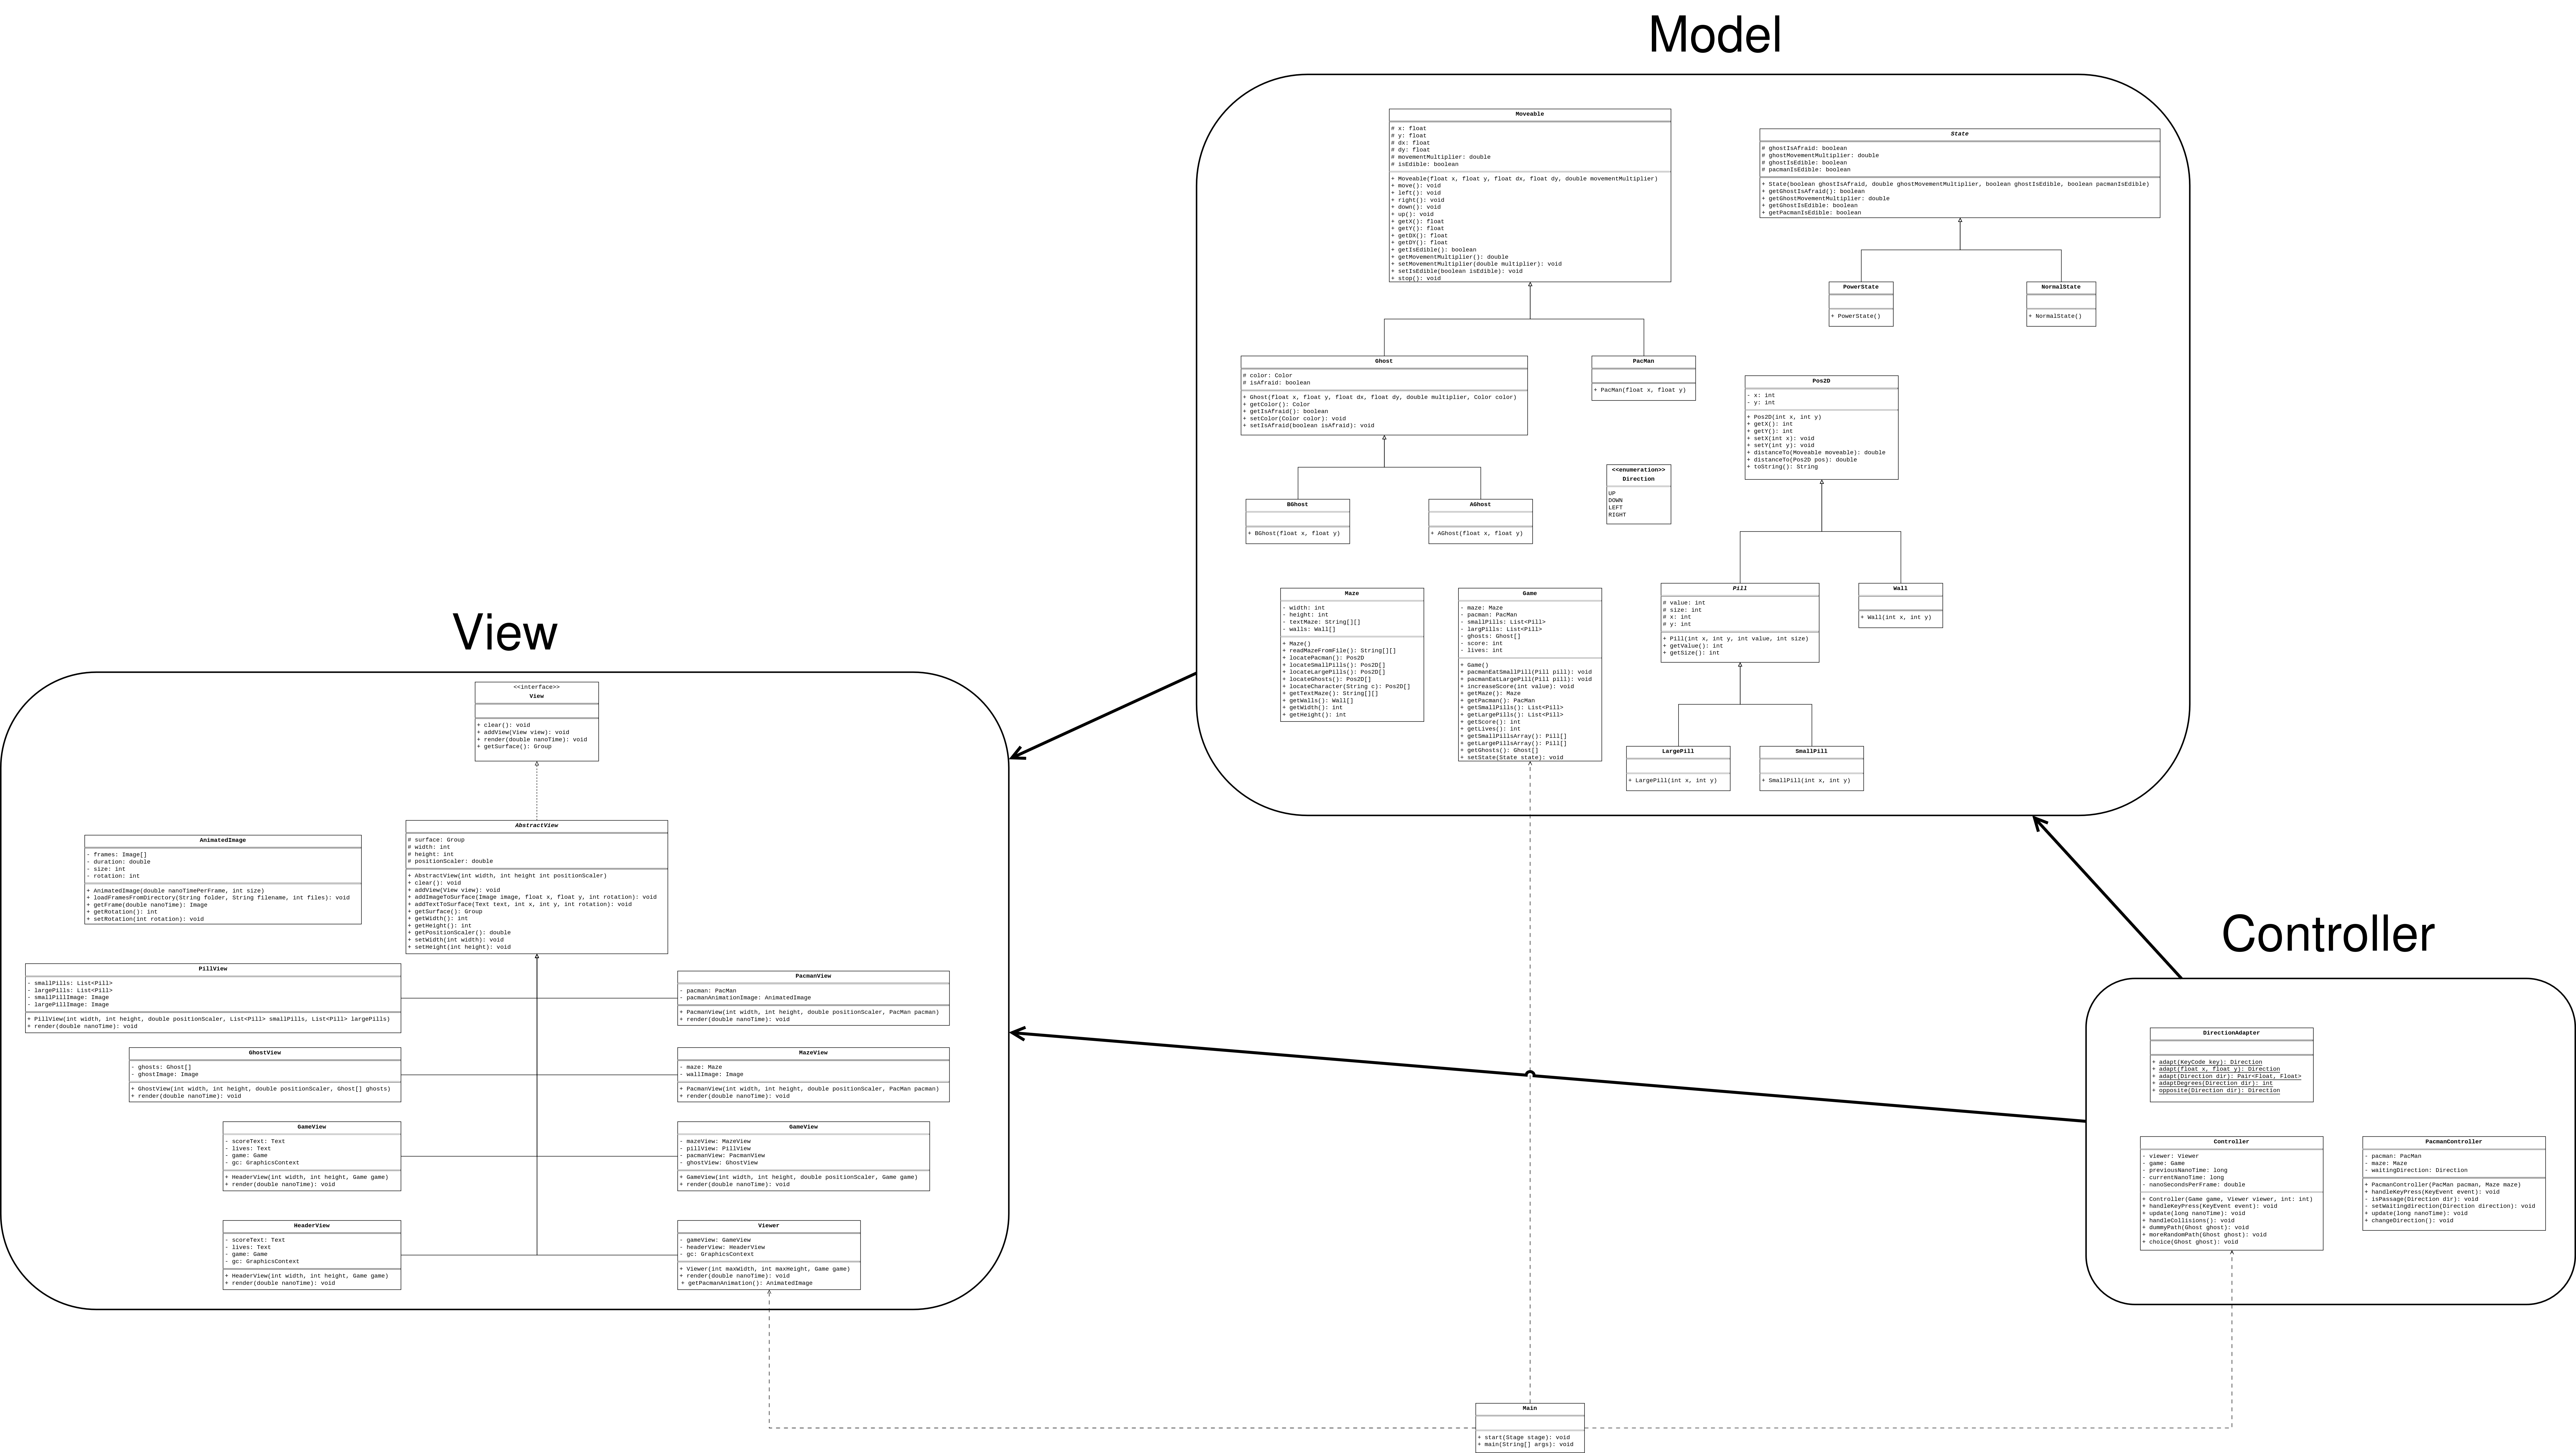
\includegraphics[width=0.95\textwidth]{figures/UML-diagram.png}
    \end{center}
    \caption{UML-diagramet til hele projektet.}
    \label{UML-diagram}
\end{figure}

Projektets design følger \textit{MVC} (Model-View-Controller) modellen. Det
vil sige at vores \textit{Model} repræsenterer hvordan PacMan spillet er bygget
op med spøgelser, vægge, piller osv. Vores \textit{Controller} som står for alt
logikken med hvordan ting skal kolliderer, og bevæge sig, og hvornår de
forskellige stadier af spillet sker. Til sidst har vi vores \textit{View} som
står for at vise spillet, med alle billederne og animationerne, samt score-tekst
og liv osv.

Designet kan ses i vores \textit{UML}-diagram (se \autoref{UML-diagram}), hvor
man kan se vi har opdelt koden i de tre dele fra \textit{MVC} modellen, samt en
\textit{main} fil som står for at starte spillet og initialisere de andre
klasser.

Vi har designet alt vores kode med fokus på \textit{indkapslingsprincippet}.
Alle felter i klasser er private, og final hvis de ikke skal ændres i. De har
også kun \textit{getters} og \textit{setters} der hvor det er nødvendigt på
denne måde benytter vi \textit{Open-Closed Principle}. Vi har også overholdt
\textit{DRY} princippet, ved at samle ens opførsel i fælles
\textit{superklasser}. Vi benytter også \textit{abstraktionsprincippet} samt
\textit{nedarvningsprincippet} som kan ses på UML-diagrammet indikeret med de
respektive pile og felter.

\subsection{Model}\label{sub:Model} % (fold)
\begin{figure}[H]
    \begin{center}
        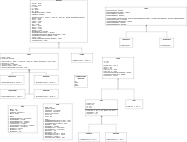
\includegraphics[width=0.95\textwidth]{figures/UML-diagram-model.png}
    \end{center}
    \caption{UML-diagram til \textit{Model} delen af projektet.}
    \label{UML-diagram-Model}
\end{figure}

I \textit{Model} (se \autoref{UML-diagram-Model}) har vi lavet et abstrakt
klasse der hedder \class{Moveable}, som er en abstrakt enhed der kan bevæge sig.
Dette tillader os at \textit{nedarve} fra selvsamme klasse når vi skal lave ting
der skal bevæge sig, som \class{Ghost} og \class{PacMan}. Udover
\class{Moveable} klassen, har vi også en klasse, \class{Pos2D}, til at beskrive
positioner som ikke skal kunne bevæge sige. Fra denne klasse kan vi så nedarve
klasser som \class{Pill} og \class{Wall}, da de kan ses som en position, men vi
også gerne vile kunne differentiere imellem dem, da de beskriver noget mere
en bare en position, især hvis vi vil udvide på hvad de er. På denne måde benytter vi
\textit{klasseafhængighedsprincippet} til at simplificerer koden, og gøre det
nemmere at udvide med nye features. Alle disse afhængigheder samt nedarvelser,
kan ses på ovenstående billede (se \autoref{UML-diagram-Model}).
% subsection Model (end)


\subsection{View}\label{sub:View} % (fold)
\begin{figure}[H]
    \begin{center}
        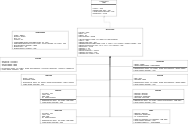
\includegraphics[width=0.95\textwidth]{figures/UML-diagram-view.png}
    \end{center}
    \caption{UML-diagram til \textit{View} delen af projektet.}
    \label{UML-diagram-view}
\end{figure}
I \textit{View} (se \autoref{UML-diagram-view}) har vi benyttet en
\textit{grænseflade} ved navn \class{View} som specificerer hvilke metoder et
\textit{View} skal have. Så har vi lavet en abstrakt klasse
\class{AbstractView}, som implementerer dette interface. Vi nedarver på denne
måde fra det abstrakte \textit{View} hver gang vi laver et nyt \textit{View} som
står for at vise andre specifikke elementer. Så kan vi lave specifikke views som
står for at tegne kun én slags ting, f.eks. \class{PacManView}. På denne måde
benytter vi princippet om et enkelt ansvar, svarende til \textit{Single
Responsibility Principle} eller \textit{SRP}.
% subsection View (end)


\subsection{Controller}\label{sub:Controller} % (fold)
\begin{figure}[H]
    \begin{center}
        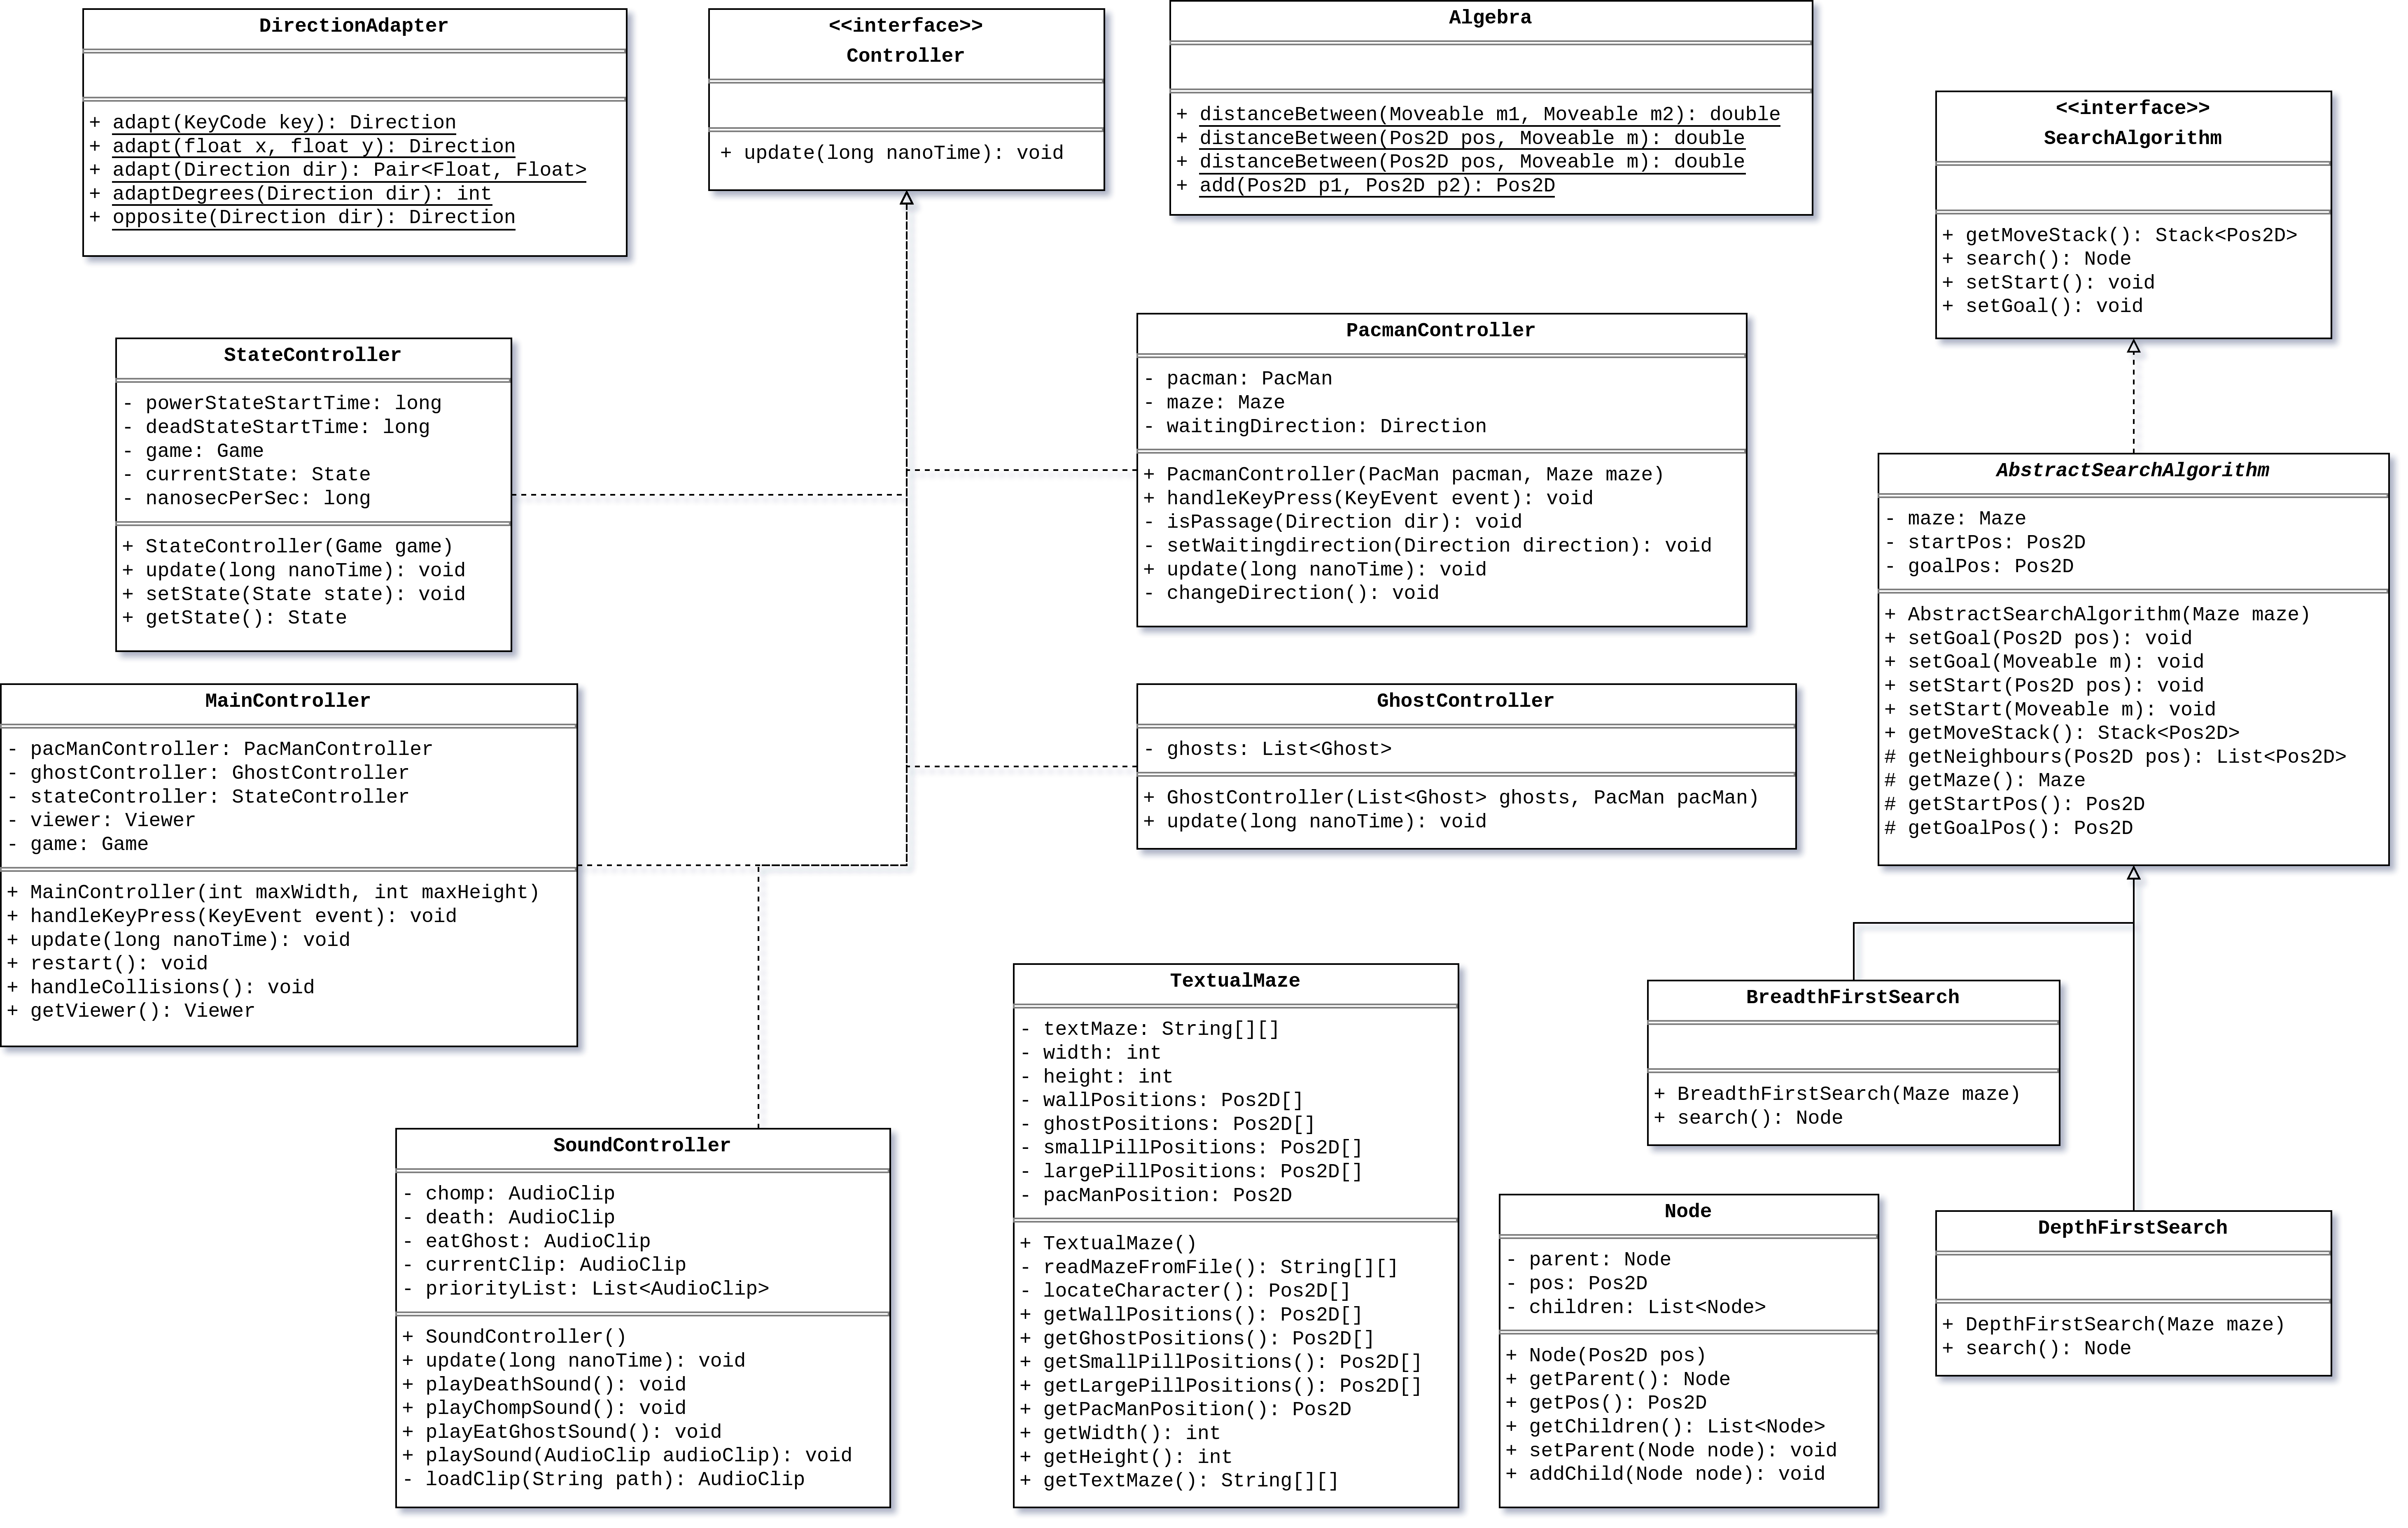
\includegraphics[width=0.95\textwidth]{figures/UML-diagram-controller.png}
    \end{center}
    \caption{UML-diagram til \textit{Controller} delen af projektet.}
    \label{UML-diagram-controller}
\end{figure}

Til \textit{Controller} (se \autoref{UML-diagram-controller}) har vi også lavet
en grænseflade, for at specificere hvad en "Controller" gør. Derefter har vi
lavet controllers til at styre henholdsvis PacMan, spøgelser og de forskellige
stadier af spillet. Med dette har vi lavet en \class{MainController} som
bestemmer hvornår alle de andre controllers skal opdateres, og hvornår vores
\textit{View} bliver opdateret.
% subsection Controller (end)


\subsection{Ændringer}\label{sub:Ændringer} % (fold)
Under udviklingsprocessen har vi valgt at arbejde i iterationer. Dette skal
forstås i den forstand, at vi først designede implementeringer via.
UML-digrammer, derefter implementerede disse designs, hvorefter vi konkluderede
på, om hvorvidt vores kodebase overholdte de ønskede designprincipper
(\textit{SOLID}). Denne process mundede ud i flere refaktoreringsprocesser, som
havde til formål, at rette op på eventuelle brud på netop disse principper.
Efter hver refaktorisering påbegyndte vi selvsamme udviklingsproces, indtil
nuværende stadie af spillet. Disse refaktoriseringer, ændrede naturligvis også
på klassernes afhængigheder mm., hvilket derfor også krævede tilpasning af
UML-diagrammet. 

Et eksempel på refaktorisering i denne proces er, at vi i
starten, blot havde sat \class{View}-klassen til at have alt ansvaret for at
tegne objekter på skærmen, samt at \class{Controller} havde ansvaret for at tage
imod input fra brugeren og styre PacMan. Resten af spillets logik i denne
iteration af udviklingsprocessen lå i \class{Maze}. Dette bryder \textit{SRP},
som derfor krævede refaktorisering inden viderudvikling.

\begin{figure}[H]
    \begin{center}
        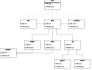
\includegraphics[width=0.95\textwidth]{figures/UML-diagram-old.png}
    \end{center}
    \caption{Det første UML-diagram til projektet.}
    \label{UML-diagram-old}
\end{figure}
I et forsøg på at simplificerer \class{Maze} delte vi den op, og lavede en
\class{Game} klasse, hvis formål var at repræsenterer spillet. På denne måde
kunne \class{Controller} stå for at håndterer alt logikken, som også er mere
typisk af en \textit{Controller} at gøre i \textit{MVC}-modellen. Med denne
ændring ville maze bare stå for at repræsenterer labyrinten. UML-diagrammet for
denne forbedring kan ses på \autoref{UML-diagram-old2}.

\begin{figure}[H]
    \begin{center}
        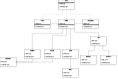
\includegraphics[width=0.95\textwidth]{figures/UML-diagram-old2.png}
    \end{center}
    \caption{Det andet UML-diagram til projektet.}
    \label{UML-diagram-old2}
\end{figure}
Siden da har vi udvidet endnu mere på projektet, og det ser nu ud som det gør på
\autoref{UML-diagram}.
% subsection Ændringer (end)

%\begin{itemize}
%  \item Inkludér et UML-diagram og en beskrivelse af jeres design.
  %\item Giv en kort beskrivelse af jeres diagram:
  %\begin{itemize}
  %  \item Hvad er de forskellige dele?
  %  \item Har I anvendt designmønstre i jeres design? I så fald, hvor i
  %  diagrammet findes disse? Det er ikke et krav at anvende designmønstre, men
  %  kan være en god idé.
  %\end{itemize}
  %\item Dokumentér designbeslutninger hvor I har anvendt SOLID, DRY, eller andre
  %OO-principper. 
%  \item Hvis I i løbet af projektet har forfinet jeres design,
%  giv da en kort beskrivelse af hvilke ændringer I har foretaget og hvorfor.
%\end{itemize}
% section design (end)


\section{Implementation}\label{sec:Implementation} % (fold)

\subsection{Spil Stadier}
For at implementere de forskellige stadier i PacMan, lavede vi en abstrakt
klasse \class{State}, som står for at definere alle de ting i spillet som kan
ændre sig i de forskellige stadier. På denne måde havde vi mulighed for at
udvide dette stadie når vi skulle lave et konkret stadie, så som
\class{PowerState}, og så blot specificere for alle attributterne deres værdier.
Så med hjælp fra \method{setState} metoden i \class{Game} kan vi ændre på
stadiet af spillet ved bare at give spillet et nyt stadie som har
\textit{supertypen} \class{State}.

Til formål for at forbedre og forsimple denne interaktion, lavede vi klassen
\class{StateController}. Denne klasse har også en metode \method{setState}, som
kalder \method{setState} i \class{Game}. Men hvis det så er en stadie, som
\class{PowerState}, der skal køre i en specifik mængde tid, så sørger
controlleren også for at håndterer det, igennem dens \method{update} metode.


\subsection{PacMan kontrol}\label{sub:PacMan Kontrol} % (fold)
Siden vi har gjort således at en \textit{Moveable}'s position er beskrevet med
decimal tal, så skal der sørges for at PacMan kan bevæge sig omkring hjørner i
labyrinten uden man sidder fast. Dette skyldes at labyrinten består af en masse
vægge på heltals-positioner, og PacMan er samme størrelse som væggene, så han
passer kun lige akkurat imellem dem.

Idéen er at man kigger frem foran PacMan for at se om der er en passage til den
side man gerne vil hen, indikeret med et tastetryk. Hvis der er en passage,
venter controlleren med at dreje PacMan indtil han er lige ved siden af
passagen. Dette har vi gjort ved at gemme retningn i et felt kaldet for
\attribute{waitingDirection}, og så hver gang \class{PacManController}'s
\method{update} metode bliver kaldt, så tjekker den om PacMan's position er en
heltalsværdi. Det må nemlig betyde at han nu står foran den passage som der
tidligere blev set. I så fald drejer PacMan nu til retningen af
\attribute{waitingDirection}. 

Der er også tilfældet hvor PacMan skifter retning til det modsatte af hvad han
bevæger sig. Så kan vi ikke kigge efter en passage der, for det vil der altid
være, og han vil dermed ikke skifte retning med det samme. Så i dette tilfælde
skifter vi bare retning ved tastetryk. Hvis det er sådan at PacMan står stille,
så er vi ikke interesseret i at kigge efter en passage, og han skal bare bevæge
sig i den retning som man trykker.

For at lave alt dette med retninger, lavede vi en \class{enum} klasse. I denne
klasse er der har vi defineret fire retninger : op, ned, højre og venstre. For
at finde ud af hvilken en af disse retninger vores tastetryk svarer til, lavede
vi også en \class{DirectionAdapter} klasse, som står for at konverterer imellem
\class{Direction} og andre representationer af en retning.
% subsection PacMan Kontrol (end)

\subsection{Spøgelses AI}\label{sub:Ghost AI} % (fold)

\subsubsection{Søge Strategier}

Vi valgte at implementere forskellige måder for spøgelserne i spillet til at
jage PacMan(spilleren). Som vores primære metoder valgte vi to kendte
søgealgoritmer, nemlig \textit{Dybde-Først søgning} \& \textit{Bredde-Først
søgning}. Vores grund for at bruge to søgealgoritmer og ikke kun én, var for at
sikre lidt uforudselighed i spillet, da spøgelserne så skulle tage forskellige
ruter mod PacMan.

\subsubsection{Node klassen}

For at kunne skabe fundamentet for at behandle vores labyrint som et binært træ
skabte vi klassen \class{Node}. Klassen består af en forældre
knude, en liste af knuder som er dets børn og en \class{Pos2D} , som er en
position i labyrinten den repræsenterer. Den første knude er roden og har ingen
forældre og ingen børn til at starte med, men den ville skulle have en start
position, svarende til et \class{Pos2D} objekt.

Metoderne i \class{Node} klassen som gav gavn til os senere var
\method{addChild}, og \method{setParent} som gjorde os i stand til at opdatere
vores binære træ. 

\subsubsection{Grænseflade for Søgealgoritmer}

Grænsefladen \class{SearchAlgorithm} er en signatur for søgealgoritmer, som
tillader os at abstrahere fra hvordan de er implementeret. Metoden
\method{getMoveStack} er vores metode for at hente den sti af positioner
spøgelserne skal gå for at nå PacMan's position. Metoden \method{search} som en
konkret søgealgortime skal implementere, hvor definitionen af algoritmen ligger.

\subsubsection{Abstrakt Søgealgoritme Klasse}

Vores plan med \class{AbstractSearchAlgorithm} som en abstrakt klasse var at, så
kunne vi bruge klassen som skabelon for andre søgealgoritmer, og implementere
\class{SearchAlgorithm} grænsefladen for at implementerer nogle af de metoder
som søgealgoritmer generelt har. Vi følte, at det var en god idé at limitere
metoderne tilgængelige for de kommende søgealgoritmer for at undgå unødvendig
kompleksitet og uforudselighed. 

En metode fra \class{AbstractSearchAlgorithm} som er essentiel for
søgealgoritmen var vores metode \method{getNeighbours}. Den er essentiel fordi
den bruges til at undersøge de fire mulige bevægelser til rådighed(op, ned,
højre, venstre) ud fra given position. Ved at gennemgå positionens naboer i
en \textit{for-løkke}, og benytte metode \method{isWallAt}, kan vi sikre at
spøgelsernes nye positioner er lovlige(der er ikke en væg) og heller ikke uden
for labyrinten.

\subsubsection{Dybde-Først Søgning}
I \textit{Dybde-Først søgning} er strategien at udforske et træ ved at
søge første venstre gren i træet og fortsætte til målet nås. Hvis målet ikke nås
i første søgning og vi i stedet når bunden af træet, så \textit{backtracker} vi
fra efterkommer knuden op mod roden og udforsker de forskellige efterkommeres
grene for at finde målet der. Hvis målet ikke findes, returneres en fejl.

For at implementere \textit{Dybde-Først søgning} brugte vi pseudokoden fra
wikipedia\cite{DFS} og oversatte den til vores program. For
at kunne bruge metoden \method{getNeighbours} fra abstrakt klassen, skal
\class{DepthFirstSearch} klassen have adgang til vores labyrint i
\class{DepthFirstSearch} konstruktøren. Ved at følge pseudokoden,
benytte \method{getNeighbours} og to metoder fra \class{Node} klassen undersøgte
vi stier af positioner til PacMan, og returnerede en stack af bevægelser som
kunne gives til \class{GhostController} og opdatere spøgelserne med
\method{update} metoden fra \class{GhostController}. 

En anden ændring er ved \class{ArrayList}'ens medfødte metode \method{contains}.
Når man i en \code{ArrayList} vil undersøge om den indeholder et objekt, kaldes
\method{contains} der bruges til at se om det objekt man passerer er i listen.
Den metode har vi måtte overskride for at passe til \class{Pos2D} objektet.
Ændringen er en \textit{for-løkke} der sammenligner \class{Pos2D}'ers X og Y
værdier.

\subsubsection{Breadth-FirstSearch klasse}

I \textit{Bredde-Først søgning} er strategien at udforske et træ ved at søge
først venstre gren og så hver gren i et træ (i samme dybde). Vi går derefter
først dybere i træet når hver gren er undersøgt, for hvert niveau. Hvis målet
ikke findes, returneres en fejl.

For at implementere \textit{Bredde-Først søgning} har vi benyttet samme metode
som til \textit{Dybde-Først søgning}, ved hjælp af den respektive
pseudokode\cite{BFS}.

Med hensyns til overskrivelse af metoder, har vi valgt at gøre det samme som i
\textit{Dybde-Først søgning}.
% subsection Ghost AI (end)

\subsection{Animationer}\label{sub:Animationer} % (fold)
Da vi gerne ville have animationer i spillet, lavede vi en klasse kaldet
\class{AnimatedImage}, som står for at repræsenterer de forskellige frames af en
animation, indlæse frames fra en sti, og ændre farver i dem hvis der er brug for
det. Med hensyn til farveændring af sprites, har vi valgt at lave et set sprites
med en specifik farve (hvis hex værdi er \attribute{\#000001}), som muligøre nem
udskiftning til en anden farven.

Når man så laver et nyt \class{AnimatedImage}, så specificerer man hvor lang tid
én frame varer i nanosekunder. På denne måde kan vi i \method{getFrame} metoden
regne ud hvilken frame vi giver, ud fra den nuværende tid som metoden får. Det
gør den ved først at regne ud hvor lang tid hele animationen tager. Derefter
finder vi hvor langt inde i den animation cyklus vi er, ved at tage den
nuværende tid modulus længden af animationen. Med dette kan vi så dividerer med
længden af én frame, og få det frame indeks som vi er nået til.

For at farve spøgelsernes animationerne de rigtige farver benytter vi vores
metode \method{replaceColorsInFrames}, som udskifter alle farver som er lig med
\attribute{fromColor} i en animations frames, og sætter dem til farven
\attribute{toColor}. Dette gør den ved at gå igennem hver frame pixelvis og
tjekke om de matcher \attribute{fromColor}, for så at udskifte det med
\attribute{toColor} på en kopi af framet, så det til sidst kan blive
overskrevet.
% subsection Animationer (end)


\subsection{Afstande \& Algebra}
For at en \class{Moveable} og en \class{Pos2D} ikke selv skal stå for at udregne
en afstand til andre objekter, har vi lavet en klasse \class{Algebra} som står
for netop dette. Argumentet for at lave en klasse som beregner netop disse ting
er at det ellers ville bryde \textit{SRP}, hvis en klasse der kun står for at
repræsenterer en position, også skulle stå for at udregne afstanden mellem
positioner.


\subsection{Labyrinten}
Til formål for at lave labyrinten til spillet, skulle vi have en måde hvorpå
det var nemt at ændre i den, og bygge den op. Derfor lavede vi den som en tekst
fil. For at læse denne tekst fil, og finde de forskellige elementer i den,
lavede vi en klasse \class{TextualMaze}. Dens formål er kun at læse
indholdet af filen, of finde positionerne af alt i filen, ved brug af metode
\method{locateCharacter}.

Udover dette har vi også lavet en klasse \class{Maze} som kun holder alle
væggene. På denne måde står \class{Maze} ikke selv for at læse en tekstfil og
kigge rundt i den, som gør at det overholder \textit{SRP}. 

\class{Wall} klassen udvider \class{Pos2D}, men med tilføjelsen af bolske
værdier der beskriver hvorvidt den har naboer i kompasretninger. Dette gjorde vi
for at gøre labyrinten mindre firkantet, ved at bruge specifikke væg billeder ud
fra hvilke af deres naboer også var vægge. Hvis der f.eks. var to vægge ved
siden af hinanden, så vil vi ikke vise en væg der hvor de rør, men i stedet
rundt om dem. Vi kom frem til at det krævede fem mulige væg billeder, og 11
cases for at opnå dette. 

% \begin{itemize}
%   \item Formålet med denne rapportsektion er at give den interesserede læser et
%   overblik over de interessante implementationsdetaljer, som er værd at kigge
%   nærmere på i jeres kodebase, samt nødvendige detaljer for at køre jeres kode.
%   \item angiv hvilken version af java i har brugt til at teste og kompilere
%   jeres kode, og inkludérkorte instruktioner til hvordan man kompilerer og kører
%   koden.
%   \item giv en beskrivelse på højniveau af interessante implementationsaspekter.
%   F.eks., aspekter, I har brugt særligt meget tid eller energi på.
%   \item Det kunne f.eks. være mere avancerede aspekter såsom hvordan I håndterer
%   AI, hvordan I håndterer spilhandlinger, animation, eller andet.
%   \item Hold beskrivelsen overordnet. Vi kan læse jeres kode for detaljerne.
% \end{itemize}
% section Implementation (end)


\section{Kvalitetssikring}\label{sec:Kvalitetssikring} % (fold)
Til fordel for at sikre, at PacMan lever op til kravsspecifikationen
(se \autoref{sec:Design}), har vi valgt at anvende unit-tests. Unit-testing
defineres i denne kontekst som test af enkelte komponenter af programmet, som
til sammen skaber det ønskede overblik.

I overenstemmelse med vores valg af unit-tests, er det også underforstået, at vi
tester i en form for \textit{White-Box} testing. Med dette betyder det, at dem der
skriver testsne (os som udviklere af spillet i dette tilfælde), kender til alt
logikken bag implementeringen. Således, har man som "\textit{tester}", altså
mulighed for at tjekke, om en given invariant for en given metode overholdes
under kørsel.

Mere specifikt; har vi valgt at benytte os af \textit{Java}'s framework
\texttt{JUnit}, som b.la. understøtter behjælpelige sammenligningsmetoder (f.eks.
\textit{assertions} via \code{assert}).

Med dette, anvender vi altså også unit-testing som middel til at krydstjekke med
vores kravspecifikation, og om disse krav samt eventuelle invarianter er
overholdt.

Med anvendelse af ovennævnte, kan fejlfindingprocessen under udviklingen, i
nogle tilfælde, forkortes markant. Man kan med andre ord, nogle gange, såfremt
man skriver tilstrækkelige unit-tests, forsimple, effektivisere, samt forbedre
design og udviklingsprocessen.

Ydermere, har vi til håndtering af versionstyring anvendt \code{git} i form af
nye branches under udvikling af nye programfunktionaliteter. Dette konstruerer
en form for automatiseret testing, da man ikke kan publicere ny funktionalitet,
før det passer med den resterende kodebase (f.eks. håndtering af
\textit{flettekonflikt} mm.). Denne form for \textit{automatiseret} testing er
også kendt som \textit{Continuous integration testing}. I det følgende, kan man
se hvorledes sådanne en unit-test kunne se ud.

Det kan eksempelvis være behjælpeligt at være sikker på, at ens metoder som er
konstrueret til at beregne distancen mellem objekter, rent faktisk returnerer
ønskede værdier. For at sikre os, at vores adhoc polymorfiske metode
\method{distanceBetween}, overholder dette, har vi valgt at konstruere følgende
unit-test:

\snippet{12}{55}{./code/AlgebraTest.java}

Man kunne derudover også have valgt at lave en form for \textit{Black-Box}
testing hvorved individer som ikke kender til kode-basen f.eks. prøver at spille
spillet og derved rapportere evt. fejl (både visuelle og logiske). Med denne
form for testing er der mulighed for at fange fejl, som man ikke selv ville have
opdaget.
% \begin{itemize}
%   \item Beskriv hvordan I har testet, at jeres kode lever op til
%   kravsspecifikationen. Har I, f.eks., benyttet unit tests? Manuelle tests?
%   \item Ville I have taget en anden tilgang til kvalitetssikring hvis I skulle
%   designe og implementere projektet forfra?
% \end{itemize}
% section Kvalitetssikring (end)


\section{Proces}\label{sec:Proces} % (fold)
\subsection{DesignFasen}
I vores første fase skulle vi blive enige om hvilken model vi ville bruge. 
\textit{Model-View-Controller}, da den virkede oplagt givet projektet natur.

\subsection{Git og samarbejde}
For at vi alle har kunne arbejde sammen på projektet, benyttede vi os af
\textit{Git} som tidligere nævnt. Brugen af \textit{Git} har sikret os at vi
kunne arbejde på det samme \textit{repository} med forskellige \textit{branches}
til hver af os. Det betød at vi hver har kunne eksperimentere med en version af
vores main-\textit{branch} uden risiko for konsekvenser til vores kodebase.
Implementationen af koden til dette større projekt løste vi bedst ved at dele
implementationsarbejdet op mellem os. Inden vi delte arbejdet op var det
nødvendigt at vi definerede vores game loop, da det ligesom fundamentet for at
vi kunne forsætte arbejdet og implementere resten af koden. Efter vi lagde
fundamentet, kunne vi arbejde både hver for sig og i grupper. Gruppearbejdet
sikrede vi alle deltog i arbejdet.

\subsection{AI}
Vi har prøvet at bruge generativ AI i vores opgave til implementations forslag
til løsninger af problemer som vi selv har haft svært ved. Mere specifikt har vi
forsøgt os med at benytte \textit{COPilot} og \textit{ChatGPT} til fordel for at
løse et "pathing" problem med vores spøgelses AI. Ingen af disse generative AI's
gav os brugbar input og vi endte istedet med at bruge \textit{VScodes}
\textit{run \& debug} funktion. Der gik vi igennem koden og rationaliserede os
frem til en løsning.

%\begin{itemize}
%  \item Arbejdede I i faser i løbet af projektet?
%  \item Hvordan gik samarbejdet, og hvordan sikrede I lige deltagelse?
%  \item Brugte I tekniske værktøjer til at få samarbejdet til at glide nemmere
%  på tværs af maskiner?
%  \item Har I brugt AI som støtte under udviklingen af jeres projekt? I så fald,
%  hvordan?
%\end{itemize}
% section Proces (end)

\section{Diskussion}\label{sec:Diskussion} % (fold)

Hvis vi skulle lave projektet om igen, så ville vi bruge mere tid på at overveje
strukturen af det hele i starten. På den måde kunne vi undgå alle de
refaktoriseringer vi har haft. Dog havde vi ikke noget erfaring med større
projekter i starten, så vi ville nok ikke have kunne forudse hvor kompleks
kodebasen blev.

Vi nåede ikke at implementere sådan at spøgelserne flygter fra PacMan når de er
bange. Dog mener vi ikke at det ville være særlig svært at lave, med vores
nuværende kodebase, da det bare ville være at ændre på hvad vi giver som målet
til søgealgoritmen i \class{GhostController}.

% \begin{itemize}
%   \item Ville I gøre noget anderledes hvis I skulle implementere projektet
%   forfra?
%   \item Var der dele af projektbeskrivelsen I ikke nåede? I så fald, hvordan er
%   disse dele kompatible med jeres design? Ville I foretage ændringer for at
%   imødekomme ændringer?
% \end{itemize}
% section Diskussion (en

\newpage
\printbibliography

\end{document}
